\documentclass[UTF8]{ctexart}

%固定图片位置
\usepackage{float}

%插入超链接
\usepackage{url}

\usepackage{tikz,mathpazo}
\usetikzlibrary{shapes.geometric, arrows}
\usetikzlibrary{calc}

%\usepackage[affil-it]{authblk}

\usepackage{listings}
%插入代码的配置
\definecolor{CPPLight}  {HTML} {686868}
\definecolor{CPPSteel}  {HTML} {888888}
\definecolor{CPPDark}   {HTML} {262626}
\definecolor{CPPBlue}   {HTML} {4172A3}
\definecolor{CPPGreen}  {HTML} {487818}
\definecolor{CPPBrown}  {HTML} {A07040}
\definecolor{CPPRed}    {HTML} {AD4D3A}
\definecolor{CPPViolet} {HTML} {7040A0}
\definecolor{CPPGray}  {HTML} {B8B8B8}
\lstset{
	language=Matlab,                                     % 设置语言
    columns=fixed,    
    breaklines = true,   
    basicstyle=\small ,
    numbers=left,                                        % 在左侧显示行号
    %frame=none,                                          % 不显示背景边框
    backgroundcolor=\color[RGB]{245,245,244},            % 设定背景颜色
    keywordstyle=\color[RGB]{40,40,255}\bfseries,                 % 设定关键字颜色
    %commentstyle=\color{red!10!green!70}\textit,    % 设置代码注释的颜色
    numberstyle=\tiny\color{darkgray},           % 设定行号格式
    commentstyle=\it\color[RGB]{0,96,96},                % 设置代码注释的格式
    stringstyle=\rmfamily\slshape\color[RGB]{128,0,0},   % 设置字符串格式
    showstringspaces=false,                              % 不显示字符串中的空格                           
    %morekeywords={True,alignas,continute,friend,register,true,alignof,decltype,goto,
    %reinterpret_cast,try,asm,defult,if,return,typedef,auto,delete,inline,short,
    %typeid,bool,do,int,signed,typename,break,double,long,sizeof,union,case,
    %dynamic_cast,mutable,static,unsigned,catch,else,namespace,static_assert,using,
    %char,enum,new,static_cast,virtual,char16_t,char32_t,explict,noexcept,struct,
    %void,export,nullptr,switch,volatile,class,extern,operator,template,wchar_t,
    %const,false,private,this,while,constexpr,float,protected,thread_local,
    %const_cast,for,public,throw,std,rand},
    emph={access,and,break,class,continue,def,del,elif ,else,%
	except,exec,finally,for,from,global,if,import,in,i s,%
	lambda,not,or,pass,print,raise,return,try,while, imshow, subplot, figure,%
    log, fft2, fftshift, abs, size, rgb2gray, imread},
    emphstyle=\color{CPPViolet}\bfseries, 
    emph={[2]True, False, None, self},
	emphstyle=[2]\color{green},
	emph={[3]from, import, as},
	emphstyle=[3]\color{blue},
	upquote=true,
	morecomment=[s]{"""}{"""},
    morecomment=[s]{\%}{},
	%commentstyle=\color{orange}\slshape,
    commentstyle=\color{red!10!green!70}\textit,    % 设置代码注释的颜色
	emph={[4]1, 2, 3, 4, 5, 6, 7, 8, 9, 0},
	emphstyle=[4]\color{red},
	emph={[5]numpy, np, plt},
	emphstyle=[5]\color{red},
	literate=*{:}{{\textcolor{blue}:}}{1}%
	{=}{{\textcolor{blue}=}}{1}%
	{-}{{\textcolor{blue}-}}{1}%
	{+}{{\textcolor{blue}+}}{1}%
	{*}{{\textcolor{blue}*}}{1}%
	{!}{{\textcolor{blue}!}}{1}%
	{(}{{\textcolor{blue}(}}{1}%
	{)}{{\textcolor{blue})}}{1}%
	{[}{{\textcolor{blue}[}}{1}%
	{]}{{\textcolor{blue}]}}{1}%
	{<}{{\textcolor{blue}<}}{1}%
	{>}{{\textcolor{blue}>}}{1},%
    %{\%}{{\textcolor{green}\%}}{1},%
	framexleftmargin=0.1mm, framextopmargin=0.1mm, frame=shadowbox, rulesepcolor=\color{black},
}



\usepackage{geometry}
\geometry{left=2cm, right=2cm, top=1.2cm, bottom=1.2cm}

%得到引用的标题内容
\usepackage{nameref} 

%添加首行缩进,两个字符
\usepackage{indentfirst}
\setlength{\parindent}{2em}

%多行公式一个编号
\usepackage{amsmath}

%文献引用,标准类型为plain
%\usepackage[hyperref=true,backend=biber,sorting=none,backref=true]{biblatex}
%\addbibresource{ref.bib}
\bibliographystyle{plain}
\usepackage{cite}

\pagestyle{plain}

%跨页表格
\usepackage{multirow}
\usepackage{longtable,booktabs}
\usepackage{supertabular}
\usepackage{makecell}

%调整itemize等的间距
\usepackage{enumitem}


\usepackage{graphicx}
\usepackage{subfigure}

%超链接
\usepackage[linkcolor=yellow,citecolor=red,backref=page,hyperfootnotes=true]{hyperref}
\hypersetup{
bookmarks=true,
colorlinks=true,
linkcolor=black
}
\usepackage{tabularx} %This package must be placed after package {hyperref}, otherwise footnote marks are NOT treated as hyperlinks.


%引入了一些改进的数学环境,如align
\usepackage{amsmath}

\title{数字图像处理报告八:小波变换与深度学习的结合}
\author{姓名:鲁国锐 \protect\newline
\and 学号:17020021031 \\
\and 专业:电子信息科学与技术}


\begin{document}
	\maketitle
	\renewcommand{\contentsname}{目录}
	\renewcommand{\listfigurename}{插图目录}
	\renewcommand{\listtablename}{表格目录}
	\renewcommand{\refname}{参考文献}
	\renewcommand{\abstractname}{摘要}
	\renewcommand{\indexname}{索引}
	\renewcommand{\tablename}{表}
	\renewcommand{\figurename}{图}
	
	
	
	\tableofcontents
	\newpage
	
	\hypersetup{
	bookmarks=true,
	colorlinks=true,
	linkcolor=red,
	urlcolor=blue
	}
	\section{题目描述}
	\indent 在之前的作业中我们探讨过如何将频率域知识运用到深度学习当中,本次作业请大家继续探索如何将小波变换与深度学习相结合进行图像处理。

			

		


	
	\section{问题背景\protect\footnotemark[1]}\label{background}
    
    \footnotetext[1]{本节的写作参考及图像来源:\par 
            \url{https://www.zhihu.com/question/22864189/answer/40772083} \par
            \url{http://users.rowan.edu/~polikar/WTtutorial.html}}
        \subsection{傅里叶变换的局限性}\label{limitation of Fourier Transformation}
            \indent 傅里叶变换作为一个提取信号频率信息的工具,有着广泛的用途。通过对一个信号进行傅里叶变换,我们可以非常清楚地看到该信号中包含了哪些频率成分。然而,很多时候,我们不仅仅想知道一个信号中包含了哪些频率,还需要知道这些频率出现的时间。
            
            \indent 于是这里引出了两个概念:\textbf{平稳信号}和\textbf{非平稳信号}。简而言之,这两种信号的区别就是:\textbf{平稳信号中各频率始终存在,不随时间变化};\textbf{非平稳信号则刚好相反}。显然,对于平稳信号,由于各频率成分不随时间改变,只需要用傅里叶变换得出其中有哪些分量及其大小相位就足以全面地描述该信号了。但是对于非平稳信号,除了知道各频率成分外,我们还需要知道每一个成分是在什么时候出现的,否则无法唯一确定一个非平稳信号。
                
			\begin{figure}[H]
				\centering 
				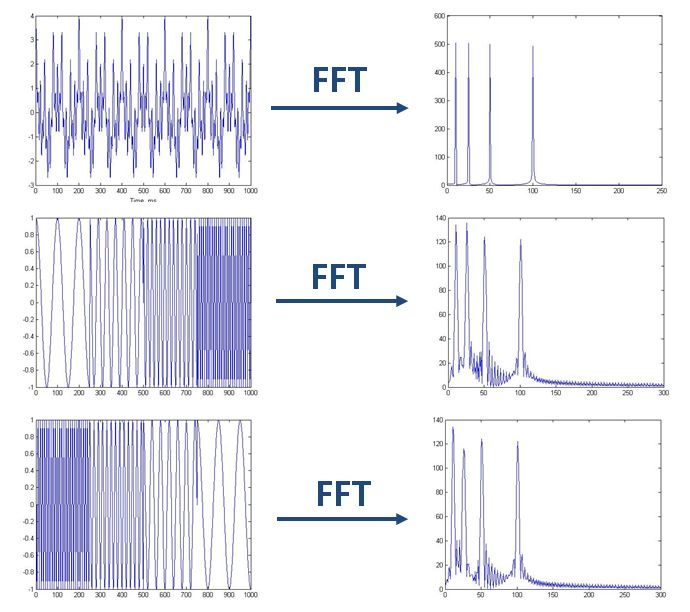
\includegraphics[scale=0.6]{non-stationary.jpg} 
				\caption{平稳信号和非平稳信号及其傅里叶变换幅频特性} 
				\label{stationary and non-stationary}
			\end{figure}                
            
            \indent 如图\ref{stationary and non-stationary}所示,最上面的一行表示的是一个平稳信号及其傅里叶变换,下面两行是两个\textbf{不同的}非平稳信号及其傅里叶变换。首先对比平稳信号和非平稳信号的傅里叶变换,可以看出非平稳信号的傅里叶变换除了有一些类似于噪声的成分外(根据\href{http://users.rowan.edu/~polikar/WTpart1.html}{第$2$条参考链接}中的解释,这是由信号从一个频率转换到另一个频率造成的),其余大体相同。接下来再对比一下两个非平稳信号的傅里叶变换,可以看出,尽管从时域上看两个信号明显不一样,但它们的傅里叶变换却几乎没有差别。显然,这样的情况使我们所不愿意看到的。
            
        \subsection{解决方案:小波变换}
        
            \indent 针对\ref{limitation of Fourier Transformation}节中所说的问题,人们想了各种解决方案,其中包括短时傅里叶变换($STFT$),即给信号“加窗”,分段做傅里叶变换。但$STFT$中的窗口大小是不变的,显然这样是无法满足分析大多数非平稳信号的要求的。于是人们又做出改进,提出了小波变换($WT$)。只不过小波变换没有在“加窗”这条路上继续走下去,而是将无限长的三角函数基换成了有限长的、会衰减的小波基(如图\ref{wavelet base}所示)。

			\begin{figure}[H]
				\centering 
				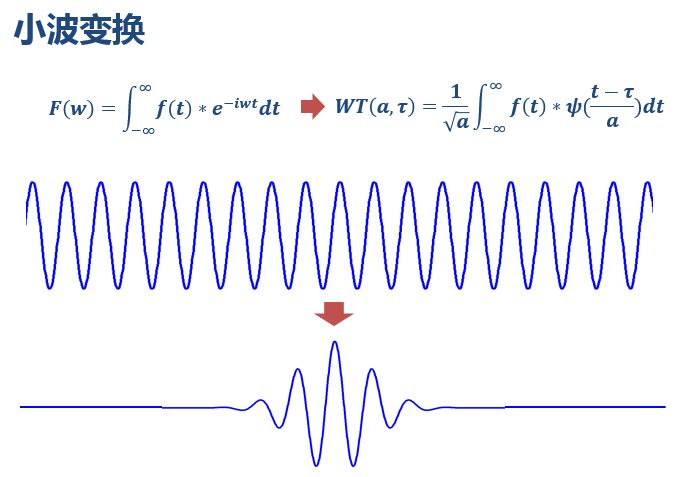
\includegraphics[scale=0.6]{wavelet-base.jpg} 
				\caption{小波变换将无限长的三角函数基换成了有限长的小波基} 
				\label{wavelet base}
			\end{figure}            
            
            \indent 通过对尺度$a$和平移量$\tau$的调整,就可改变基函数的频率(与尺度成反比)和作用的时间(对应于平移量)了。相应的,变换后的结果$WT\left( a, \tau \right)$也就可以反映出信号所包含的各频率成分及其出现的时间了。
            
            \indent \textbf{个人理解,如果用一首乐曲来比喻的话,傅里叶变换会给出这首曲子中出现了哪些音符(频率),而小波变换则能够直接给出这首曲子对应的乐谱(频率对应音符,时间对应音符出现的顺序及节奏)。}
            
    \section{小波变换与深度学习的结合:构建超分辨率图像}\label{combination of WT and Deeplearning}
        
        \indent 关于小波变换与深度学习结合的文献似乎并不多,而在完成本次报告的过程中,搜集到的文献主要又都集中在超分辨率图像的构建上\cite{deng2019wavelet, zhong2018joint, huang2017wavelet, gao2016hybrid},可见小波变换与深度学习的结合在该领域上确实有优势。故在这一小节中,我们将专门介绍小波变换与深度学习在构建超分辨率图像中的应用。
   
        \indent 另外再记录一下本次报告中文献的搜集方式:
        
    			\begin{enumerate}[leftmargin=50pt]
    				\item 首先在网上找到了一篇$ICCV2019$的论文;
    				\item 然后在论文中搜索关键词“$wavelet$”,在其参考文献中找到所有包含该关键词的论文;
    				\item 因为深度学习是在$2012$之后开始变得广为人知的,所以剔除所有早于$2012$年的文献;
    				\item 再依次去读剩下论文的摘要,判断是否符合本次报告的要求;
    				\item 找到符合要求的文献后,再对该文献重复上述步骤,最终找到本次报告中用到的$4$篇论文。
    			\end{enumerate}
        
        \subsection{用深度学习的方法来预测小波系数}
        
            \indent 在\cite{zhong2018joint, huang2017wavelet}两篇文献中,都采取了将低分辨率图像作为输入,用深度学习的方法预测其对应的高分辨率图像的小波系数来达到提升结果质量的目的。仔细阅读之后发现,这两篇论文在大体的流程设计上都比较相似,具体可以描述为:
    			
                \begin{enumerate}[leftmargin=50pt]
    				\item 输入一张低分辨率图像,得到其一组特征映射($feature\ maps$);
    				\item 将得到的特征映射输入到一组子网中,用于预测出高分辨率图像的小波系数;
    				\item 根据得到的小波系数重建出高分辨率图像。
    			\end{enumerate}
                
            \indent \cite{gao2016hybrid}中也用到了通过神经网络生成小波系数的方法,但其具体方法我并没有看懂,只能介绍到这里。
                        
        \subsection{用小波变换来分离“客观质量”和“感知质量”}
            
            \indent 在\cite{deng2019wavelet}中,作者指出,在过去的超分辨率图像构建任务中,$GAN$的对抗损失函数虽然可以促使网络生成高质量的细节,但是这些细节不在正确的位置上,最终会导致图像中出现很多伪影,出现失真。同时文中也指出,由于客观质量($objective\ quality$)和感知质量($perceptual\ quality$)受不同因素影响,如果将它们作为一个整体进行优化,将很难在两者之间找到平衡。于是作者通过使用小波变换来分离出影响客观质量和感知质量的因素,然后对其分别进行提升。
            
            \indent 具体而言,可以用小波变换将图像分解为低频子带和高频子带,其中低频子带主要影响客观质量,高频子带主要影响感知质量。然后用一个增强网络来优化低频子带,用小波域风格迁移($wavelet\ domain\ style\ transfer$)方法来提升高频子带的质量。这样做可以使结果在客观质量和感知质量之间达到一个更好地平衡。
            
%    			\begin{figure}[htbp]
%    				\centering 
%         			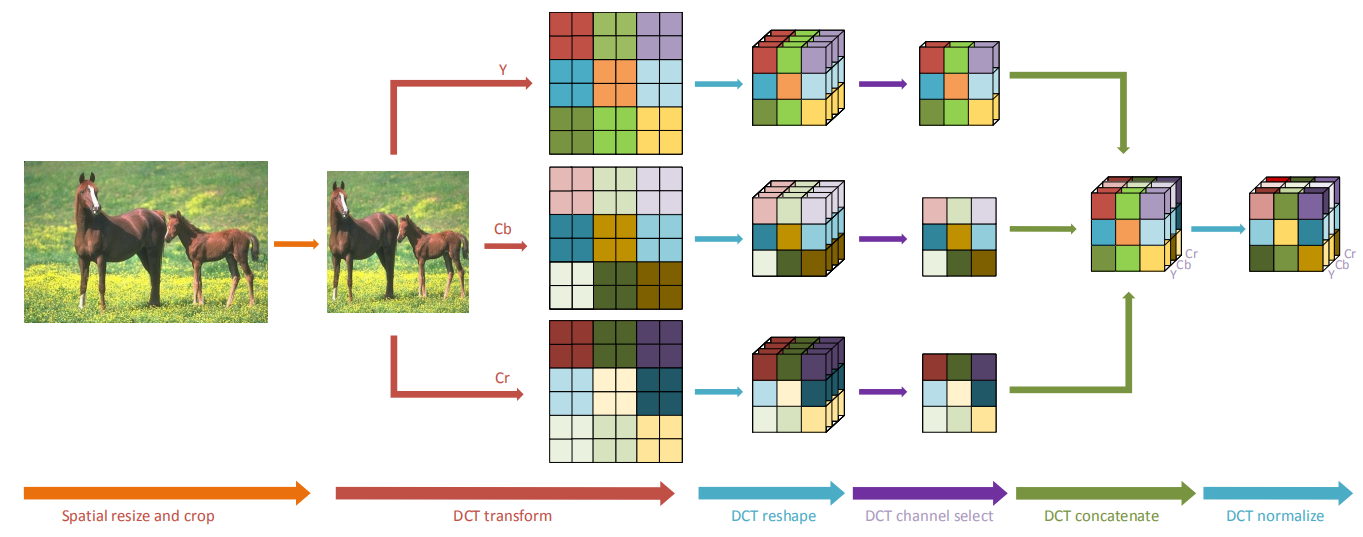
\includegraphics[scale=0.5]{pre-processing.png} 
%    				\caption{预处理流程示意图} 
%    				\label{pre-processing}
%    			\end{figure}
  
            
%        \nocite{digit_image_Gonzalez}
%        \nocite{signal_and_system}
%        \nocite{discrete-time_signal_processing}



		

            


%			\indent 采取\ref{数字相机成像原理}节的方式,我们也可以把线性扫描相机的原理概括为以下$3$个步骤:
%			\begin{enumerate}[leftmargin=50pt]
%				\item 由条带传感器成像,给出一幅图像一行(或一列)的像素值;
%				\item 沿垂直于传感器带的方向移动一小段距离;
%				\item 重复步骤$1$和步骤$2$,直至整幅图像全部成像完毕。
%			\end{enumerate}

%		\begin{enumerate}[leftmargin=50pt]
%			\item 所成图像在垂直方向上的大小不受限制;
%			\item 能够通过提高扫描频率达到非常高的分辨率;
%			\item 使用起来灵活方便等
%		\end{enumerate}
		
%	\section{实验验证}
%        \subsection{实验思想}
%            \indent 从前面的分析可以看出,频谱图上的谱线与空间域中像素变化的方向及剧烈程度有关。从这个角度出发,如果把空间域图像转一个角度,频谱图中的谱线相应地也应该旋转相同的角度。我们将在之后的两个小节中对这个猜想进行验证。
%        \subsection{实验代码}
%            	\begin{lstlisting}[language=Matlab,caption={实验代码},label={broadcast.cpp}]
%% reference: https://blog.csdn.net/jiugedexiaodi/article/details/79705308
%
%
%
%img = imread('C:\Users\Asus-\Desktop\数字图像\report\04\rotate45.png');
%img = rgb2gray(img);
%
%% 将图像的数据格式转换为double型的,此时图像的数值范围由原来的[0,255],
%% 变成了[0,1],其实不进行转换的话,也可以进行傅里叶变换,
%% 只是傅里叶变换后的图像会有所不同
%img=im2double(img);
%
%% size(img)
%
%F = fft2(img);
%F = fftshift(F);
%F = abs(F);
%
%% 傅里叶变换后模值差异非常大,低频直流远远大于高频
%% 不加这一句变换后的结果只能看到中间有一个亮点
%T = log(1+F);
%figure(1)
%subplot(1, 2, 1)
%imshow(img)
%subplot(1, 2, 2)
%% 后面的[],表示对图像做了一个类似于归一化的操作,
%% 防止傅里叶变换后模值差异太大
%imshow(T, [])
%            	\end{lstlisting}
                

        
%            \begin{figure}[htbp]
%            	\centering 
%                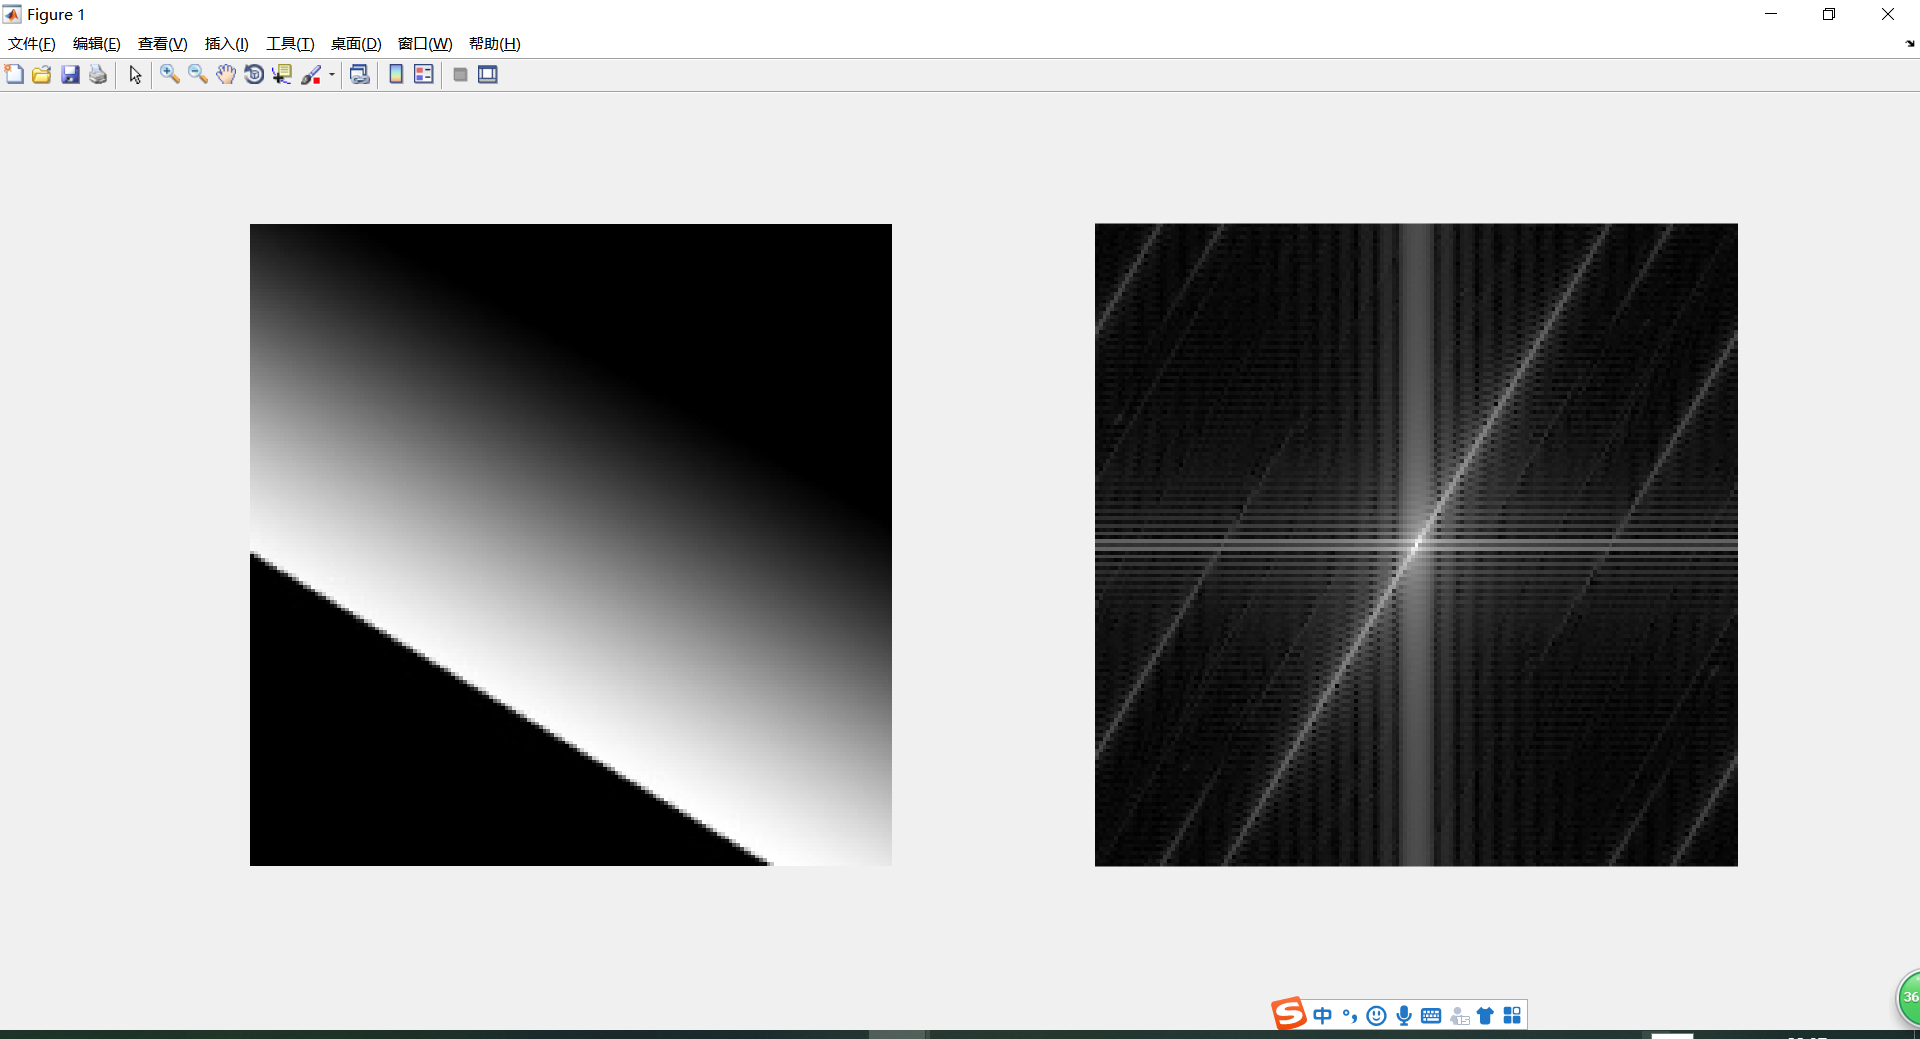
\includegraphics[scale=0.4]{result.png} 
%            	\caption{实验结果} 
%            	\label{result}
%            \end{figure}

            


	\section{总结}
    
		\indent 本次报告大概是自学这门课以来难度最大的一次了,尽管将大多数时间都花在了学习小波变换上,但在阅读论文时还是遇到了不小的阻力。一方面小波变换本身理论性很强,难度较大,通过自学只是了解了一些皮毛,论文中用到的很多知识点都未曾接触过;另一方面,目前对于深度学习更深入的知识掌握得还相当有限,也使得阅读论文的难度加大。
        
        \indent 不过,虽然有很多地方不明白,但在阅读这些文献的过程中,也能明显感受到小波变换能够在很大程度上反映出图像质量,尤其是一些细节上的信息,这对于构建超分辨率图像有着相当重要的意义。同时也可以想见,小波变换在其它相关领域,如图像修复、图像增强等方向上,也应当能起到非常重要的作用。
%			\begin{figure}[H]
%				\centering 
%				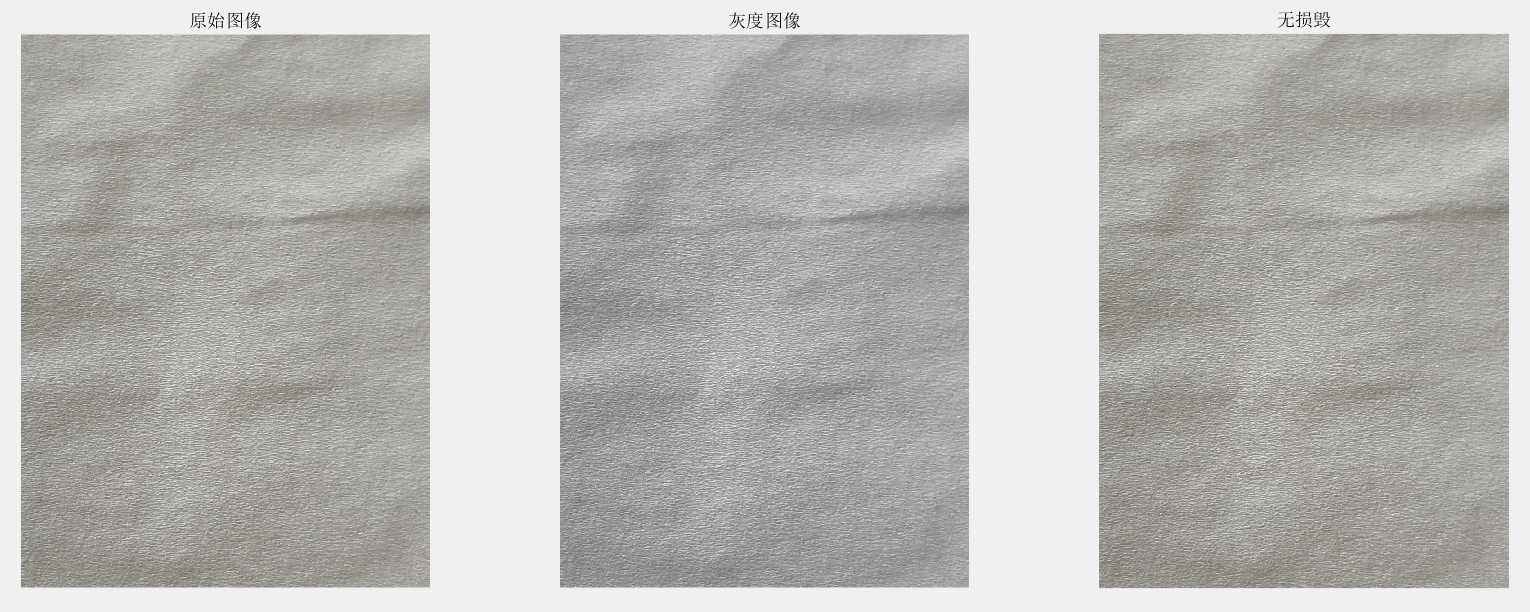
\includegraphics[scale=0.4]{res4.png} 
%				\caption{结果4} 
%				\label{res4}
%			\end{figure}
		

		
%			\begin{figure}[H]
%				\centering 
%				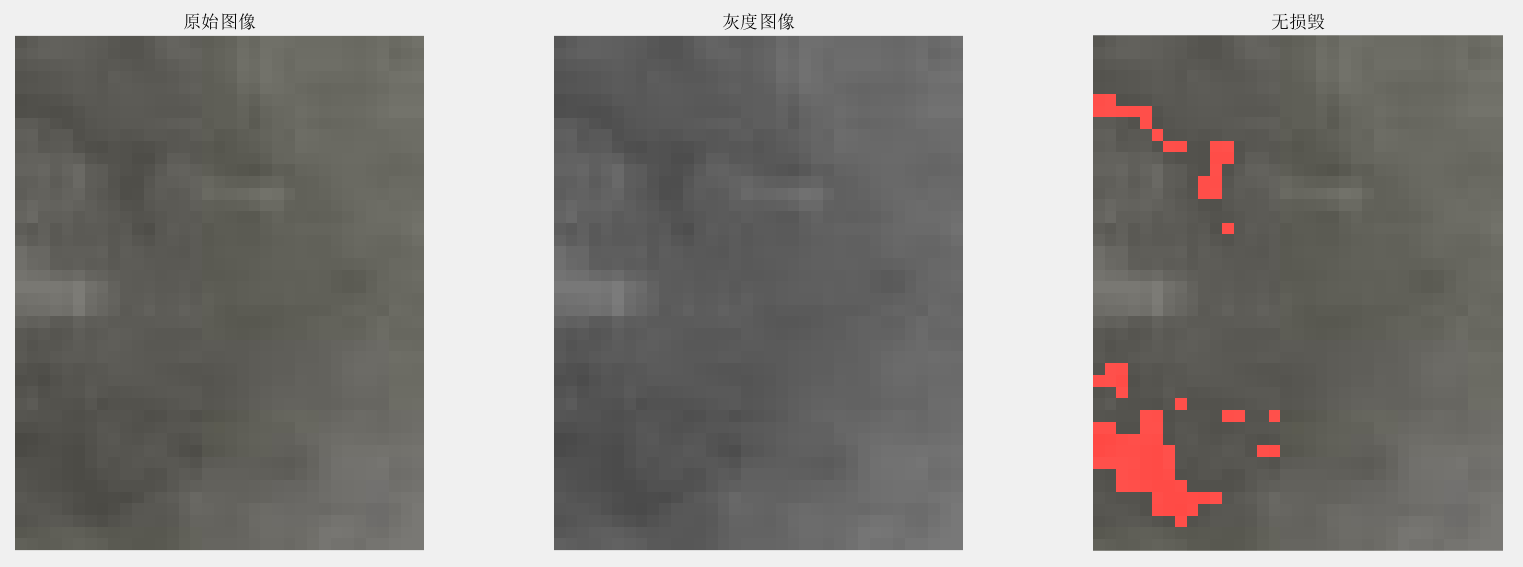
\includegraphics[scale=0.4]{res6.png} 
%				\caption{结果6(截取自结果5的阴影部分)} 
%				\label{res6}
%			\end{figure}
	
	
% 中文文献多个作者用中文逗号“,”连接
%\bibliography{ref.bib}
%\bibliographystyle{abbrv}
\bibliography{ref.bib}


\end{document}